\documentclass{article}
\usepackage[utf8]{inputenc}

\title{RodCutting Problem}
\author{Cismaru Razvn}
\date{June 2018}

\usepackage{natbib}
\usepackage{graphicx}

\begin{document}

\maketitle

\section{Problem Statement}
RodCutting Problem\\ Given a rod of length n inches and an array of prices that contains prices of all pieces of size smaller than n. Determine the maximum value obtainable by cutting up the rod and selling the pieces. 
\\

\begin{figure}[h!]
\centering
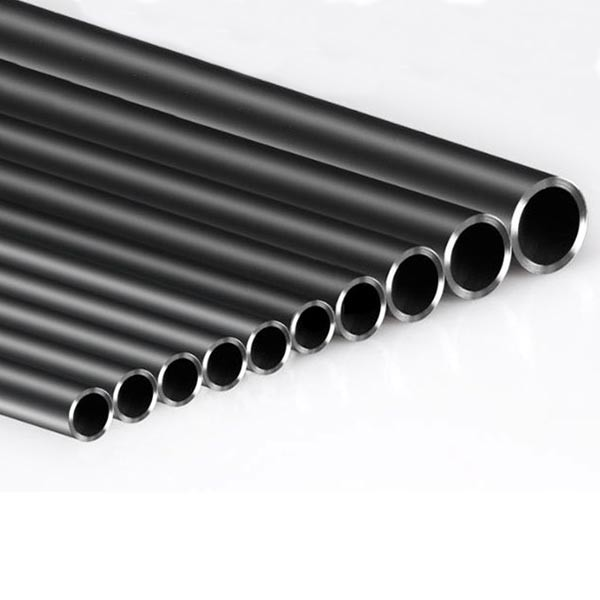
\includegraphics[scale=0.4]{teava.jpg}
\caption{The core formula}
\label{fig:universe}
\end{figure}

\section{Understanding the problem}
``So we have the lenght of the rod and the prices witch indicates all the values we can sell rod to the customers starting with 1 meter to n meters.
\\ I think this problem can be made with a lot of variants, but the one that I came with is about dynamic programing and will be based on the Figure 2 formula and the final principal code will have a complexity of O(nto2),  while the second one will be less efficent and will not be able to solve for example a rod with lenght 200. '' 

\begin{figure}[h!]
\centering
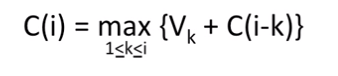
\includegraphics[scale=0.6]{formula.PNG}
\caption{The Rods we want to cut}
\label{fig:universe}
\end{figure}




\section{The generator used}
``For this problem, I needed to generate first a number and then n random numbers from 0 to infinity. As I thought that the price of a meter of rod (witch is not made of gold) would not cost more then 5 euro, the generator will come first with a number between 1 and 5 and then generate the next ones adding to the previous one a value between 1 and 5\\ The generator uses extension time.h and then uses srand function PROCENT   by n + 1 to give random values between 1 and n '' \\\\\\\\\\\\





\section{Application in real life}
``As this problem is a pure example of dynamic programing and the prices in real life won't be bigger if we buy more, I consieder that this program is just an example based on real life situation and can be continued and improved to become a functional program that may help us buy more efficent :) " \\\\\\\\\\\\\  \




\section{Exemple of running the program}
\begin{figure}[h!]
\centering
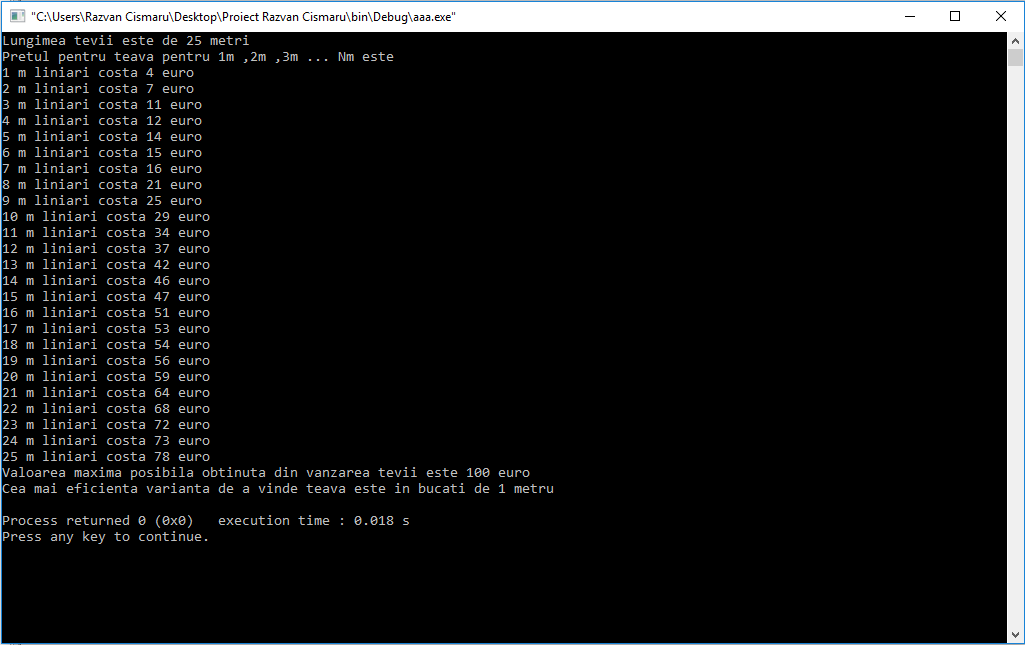
\includegraphics[scale=0.6]{exemplu.PNG}
\caption{Example}
\label{fig:universe}
\end{figure}
``As we can see, the program works and has some extras witch says if the most efficent way of selling the rod is by selling meter by meter or if it is the sittuation that the most efficent way to sell it is by not cutting it at all'' \


\section{Conclusion}
``Working  on  this  project  was  a  really  unique  experience  for  me,  since  it  was truly a challange, both in terms of research and understanding of the topic, aswell as in the implementation part.  I can say that i have learned some new things making this project and that it has started the interest of making a code that may help me do something easier or even my parents with their business.\\


\section{The Code}
``The lines of code are shown in Fig 4 '' \
\begin{figure}[h!]
\centering
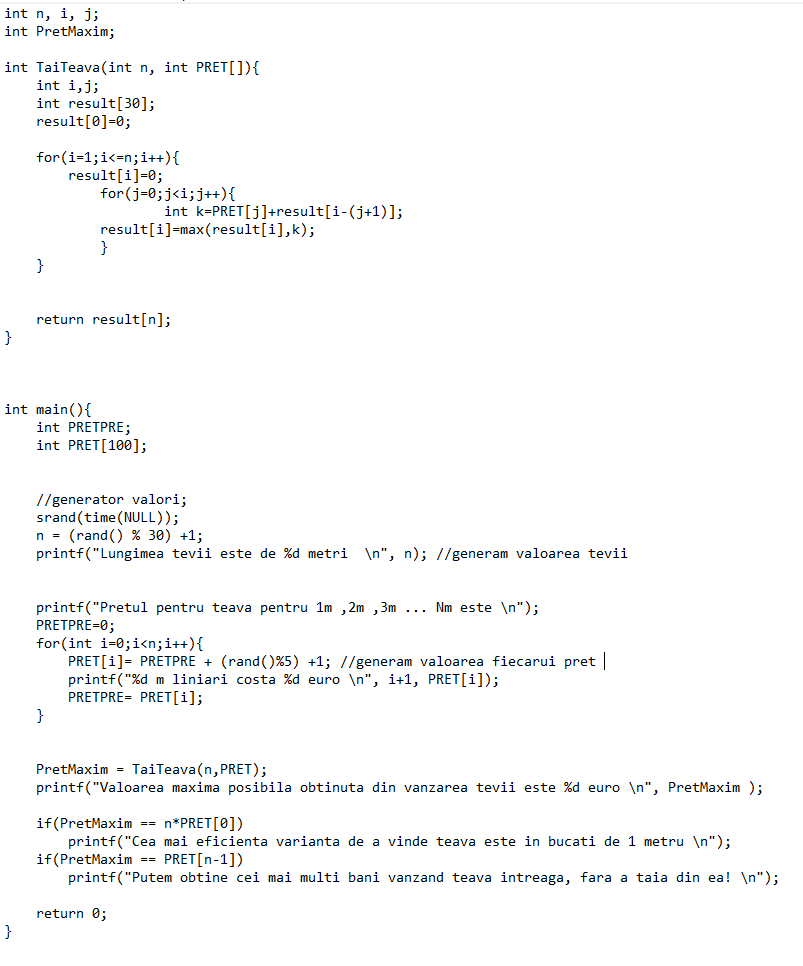
\includegraphics[scale=0.6]{codec.PNG}
\caption{The Code}
\label{fig:universe}
\end{figure}



\end{document}
